\chapter{The BB84 Simulator}
\label{chap:implementation}
% Talk about current arena of quantum computing
There are already several quantum computers available to the public in the form of APIs.
These APIs allow users to simulate and perform quantum computation by sending requests to a quantum processing unit (QPU) \cite{qiskit}. 
O'Riely has even recently released a textbook on Qiskit, IBM's quantum programming library\cite{pqc}.
Qiskit allows programmers to simulate and test quantum programs locally before running the code against IBM's cloud quantum computer \cite{qiskit}. 
Other platforms, such as D-Wave's quantum annealing API, let programmers explore other quantum computation paradigms, not just the imperative quantum paradigm we have discussed here. 

These advancements make quantum computation ever more accessible to the general public.
However, there are still many limitations; compute-time access must be shared, the number of qubits a user can control is limited, and networking is currently not possible using public quantum computing APIs.
This leads to the further development of efficient quantum simulation libraries such as Simulaqron, a quantum networking library, and qrack, an efficient quantum simulation library \cite{qrack}.
Due to the number of qubits and networking required to run the BB84 protocol, all applications presented by this thesis have been written using quantum computation simulators such as those aforementioned. 


% Discuss simulaqron
\section{Simulaqron Quantum Network Simulator}
Simulaqron is a quantum network simulation library that allows the programmer to define networked clients and have let client programs manipulate and exchange simulated qubits \cite{simulaqron}.
An instance of Simulaqron acts as a quantum server in the simulator.
It serves as both the public quantum channel host and the quantum computer that creates and distributes the qubits to each party.
% How does it work

Simulaqron is architected as a simulated QPU singleton, that is to say it stores all qubits in the network.
Simularon acts as an interface and adapter to the simulated QPU backend, which can be configured.
This allows the user to chose a backend that optimizes the sorts of operations they will perform.
Though there are currently no backends for simulaqron that perform quantum computations on a true QPU, one could be written \cite{simulaqron}.

\begin{figure}[htp]
\centering
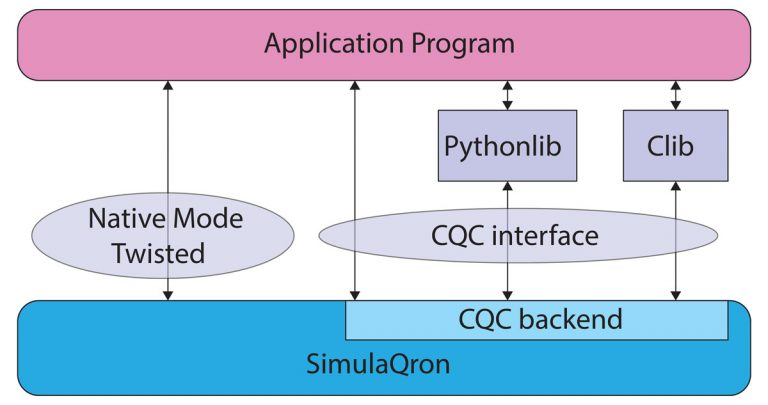
\includegraphics[scale=0.30]{images/CQC_schematic.jpg}
\caption{Schematic of the simulaqron stack.}
Source: http://www.simulaqron.org
\label{}
\end{figure}

The quantum network connected to simulaqron is also configurable. 
The programmer may specify a network topology graph, client nodes and connections, and a client can connect by identifying itself as a node in the topology.
Clients connected to a simulaqron server can request and manipulate qubits kept on the server, and the server maintains qubit information such as state and ownership.
This network can be accessed through several methods: Native Mode, which is designed for building interfaces to simulaqron, and the CQC interface, which is what was used in the BB84 simulator.

\subsection{The CQC Interface}
% Discuss CQC
The CQC interface library is the main method with which a program interfaces with a simulaqron server.
The interface itself is a client and server side implementation of the command pattern, with friendly libraries available in Python, C, and Rust \cite{simulaqron}.
For the purposes of this thesis, the Python library will be the subject of discussion.
% Talk about the interface
The client side library behaves in code like a local QPU object, allowing users to create qubits and manipulate them, making it very accessible.

% Discuss library
To use the CQC in a client there must be a simulaqron already running locally or at a known address.
A connection object must first be instantiated, since all quantum operations are performed server-side.
This can be done with 
\code{cqc = CQCConnection("Client\_name", socket\_address=("1.1.1.1", 8801))}
or, preferably, using the following syntax: 
\code{with CQCConnection("Client\_name") as cqc:}.
If the socket address argument is omitted then the connection targets localhost \cite{simulaqron}.
With a CQC connection instantiated, a client can request qubits from the server, \code{q = Qubit(cqc)}.
All new qubits are initiated to the state $\ket{0}$.
Once the server has responded with a new qubit, the client can apply quantum gates to it
For example, they can use \code{q.H()} to apply the Hadamard gate and \code{q.Z()} to apply the Z gate. 
Once the qubit is in the desired state, it can be measured with `result = q.measure()`, at which point the function returns a 1 or 0 and the qubit is discarded by the server.
It is notable that the qubit is not discarded if the user passes the flag \code{inplace=True} to \code{measure()} , but this flag is false by default.

The interface allows for communicating classical information as well.
The functions \code{sendClassical()} and \code{recvClassical()} will send and receive an array of bytes between two client applications. This is especially useful when communicating information about quantum protocols.

A programmer can send qubits between clients as well using this interface.
Consider a client, Alice, that wants to send the client Bob a single qubit.
This can be accomplished as shown in listing ~\ref{listing:cqc_example}.
Although, when using the interface, it is impossible to know the state of a qubit if you do not measure it yourself, it is noteworthy that since the connection object requests the measurement from the server, and the server responds with the result, a malicious party could use use packet sniffing to obtain the value of a qubit measurement.

\noindent
\begin{minipage}{\linewidth}
\begin{singlespace}
\lstinputlisting[label=listing:cqc_example, caption=An example usage of sending a qubit between two clients in CQC.]{code/cqc_example.py}
\end{singlespace}
\end{minipage}

As a point of verification, CQC was used to test the randomness of simulaqron.
While it is not true-random, it did provide satisfactory results.
In a trial of measuring encoding 100 qubits into the state $\ket{+}$, and measuring them in the standard basis, as a 0 or 1, 10,000 times, we found that 50\% of the qubits were 1, on average, with a standard deviation of 4\%. 
The same experiment was repeated using python's standard library random number generator, which produced the same mean and standard deviation.
This lead us to conclude that the two forms of random number generation were comparable. If the measurements were performed by an actual QPU on real qubits, they would, of course, be true-random.


\section{BB84 Simulator Library}
% Discuss bb84
The BB84 QKD protocol can be implemented using CQC, as it has all the necessary quantum functionality.
During the key exchange all quantum and classical communication is done using \code{cqc.sendQubit()} and \code{cqc.sendClassical}, respectively.
As previously mentioned, in this form, the quantum channel is still vulnerable to packet sniffing, but once the key is generated the symmetric encryption cannot be broken, if used correctly \cite{cryptography}.
% Reiterate the protocol
The BB84 can be broken into into Alice and Bob's respective responsibilities.
Since each client will have to operate independently, we will need to examine them each individually.

\subsection{Alice}
Alice first has to connect to the server.
As previously shown, this can be done with \code{with CQCConnection("Alice") as Alice:}.
Having connected to simulaqron, Alice must generate $N$ random bits, where $N \geq 3k$, $k$ = desired key size.
This is done twice, once for the key's bit values and once for the bases.
Since the qubits can be used a random number generator, this is done as shown in listing ~\ref{listing:q_random_gen}.
\begin{figure}[htp]
\begin{minipage}{\linewidth}
\begin{singlespace}
\lstinputlisting[label=listing:q_random_gen, caption=Randomly generating N bits using the CQC library.]{code/q_random_gen.py}
\end{singlespace}
\end{minipage}
\end{figure}
Next, Alice encodes the bits into qubits, choosing the basis to use according to that index on the basis bitvector as shown in listing~\ref{listing:q_encoding}.
\begin{figure}[htp]
\noindent
\begin{minipage}{\linewidth}
\begin{singlespace}
\lstinputlisting[label=listing:q_encoding, caption=Alice encodes a list of bits into qubits.]{code/encoding_example.py}
\end{singlespace}
\end{minipage}
\end{figure}
Alice then sends all the qubits to Bob.
Once Alice receives Bob's chosen bases for measurement, she can perform a NXOR between her and Bob's bases.
The result of this operation is a bitvector representing those qubits which were both encoded and measured using the same basis: \code{correct\_bases = \textasciitilde bobs\_bases \textasciicircum alices\_bases}.
This new bitvector of correct bases is sent back to Bob, and Alice discards all qubits that were measured in the wrong basis: \code{key = [bits[i] for i in range(N) if correct\_bases[i] == 1]}.
Alice then receives some of the bit values from Bob's final key.
In this implementation all bits except the last $k$ are exchanged. 
Alice then XORs the two verification bitvectors together; if the result of the XOR is non-zero then Alice knows there has been interference \cite{qc:agi}.
Alice notifies Bob of whether or not interference was detected.
If there were no errors in the compared bits, Bob is sent an OK and the compared bits are discarded from the key.
If there was an nerror between the compared bits, Bob is notified that there were differences, the process is aborted, and an exception is raised.
If the process was not aborted, the remaining bits are the final key to be used in encryption.



\subsection{Bob}
Bob must first connect to the simulaqron server.
Bob listens on the quantum channel for Alice to start sending qubits.
Bob then receives $N$ qubits from Alice and measures each qubit in a randomly chosen basis, as shown in listing ~\ref{listing:measure_random}.
\begin{figure}[htp]
\noindent
\begin{minipage}{\linewidth}
\begin{singlespace}
\lstinputlisting[label=listing:measure_random, caption=Bob measures received qubits in randomly chosen bases.]{code/measure_random.py}
\end{singlespace}
\end{minipage}
\end{figure}
With the bases chosen and qubits measured, Bob sends the bases to Alice in the form of a bitlist: \code{Bob.sendClassical(Alice, bases[:])}.
Next Bob receives the list of correct bases from Alice: \code{correct\_bases = BitVector(bitlist = Bob.recvClassical())}.
Bob, like Alice, drops all bits from his key if it was not measured in the correct basis: \code{key = [bits[i] for i in range(N) if correct\_bases[i] == 1]}.
They remaining bits should be the same for both Alice and Bob. 
To verify this, Bob sends all the bits except for the final $k$ to Alice: \code{Bob.sendClassical("Alice", key[:len(key)-k])}.
Bob then waits to receive the verification confirmation from Alice.
If the verification is an OK, then Bob sets the key to the last $k$ bits of the key with \code{key = key[k:]}, otherwise the process is aborted and an exception is raised.

Both Alice and Bob's functionalities have been abstracted into two functions, \code{initiate\_keygen()} and \code{recv\_keygen()}, respectively.
These functions, and all helper functions, have been published as  Open Source Software under the MIT license \cite{libbb84}.

\subsection{Eve}
Adding an eavesdropper into the mix is not technically possible using the simulaqron library \cite{simulaqron}.
This is because messages are send directly to the target recipient, and the library does not have functionality to go through a third party silently.
However, the eavesdropping behavior can be achieved by having both Alice and Bob use Eve as a proxy.

If Eve does not manipulate the qubits en route, acting as an unmalicious proxy, she can easy accomplish this by having both Alice and Bob list her as the recipient for qubits, while she runs code shown in listing ~\ref{listing:good_proxy}.
\begin{figure}[htp]
\noindent
\begin{minipage}{\linewidth}
\begin{singlespace}
\lstinputlisting[label=listing:good_proxy, caption=Eve acting as an unmalicious proxy between Alice and Bob.]{code/good_proxy.py}
\end{singlespace}
\end{minipage}
\end{figure}
If, however, Eve chooses to maliciously attempt to measure the qubits, this can be accomplished as shown in listing ~\ref{listing:malicious_proxy}.
\begin{figure}[htp]
\noindent
\begin{minipage}{\linewidth}
\begin{singlespace}
\lstinputlisting[label=listing:good_proxy, caption=Eve acting as an malicious proxy between Alice and Bob.]{code/malicious_proxy.py}
\end{singlespace}
\end{minipage}
\end{figure}
Although, in theory, there is a small chance that Eve is not detected, in 1000 empirical tests Eve's measurements were detected in ever instance.

\section{BBChat Messaging Software}
% Discuss chat program
As a proof of concept, BBChat, a peer-to-peer and end to end encrypted messaging application, was written to use the BB84 simulator to establish a symmetric encryption key \cite{bbchat}.
It was preferentially written as a terminal application, with text-based user interface (TUI).
BBChat requires both clients to specify whether or not they are the initiator, ``Alice", or the receiver, ``Bob", in the key generation process.
This is done with by starting the program with the command line flag \code{-i}, for ``initiator".

Upon starting, the program immediately calls \code{initiate\_keygen()} or \code{recv\_keygen()}, depending on if the program is the initiator or not.
Throughout the process of key generation, the BB84 library outputs log information to a ``quantum log", which is presented in a pane of the TUI. 
This allows the user to view the BB84 in real time, and gain better insight into its intricacies.
If too few bits are in the final key, too few bases were correct between Alice and Bob, then the key generation is restarted.
If Alice and Bob exchange verification bits and there is a difference between the bits, the user is notified in the quantum log, and the key exchange is aborted \cite{bbchat}.
If the key generation is successful, both clients open a direct TCP connection to each other.
The users can now send symmetrically encrypted messages to each other. 

